% Problem 13: Complex Numbers and Polynomial Geometry
\begin{problem}[Complex Numbers and Polynomial Geometry]
Let $n$ be a positive integer such that $n \geq 2$. Consider the complex equation $z^{2n} - 1 = 0$, whose roots are represented by the vertices $P_0, P_1, P_2, \dots, P_{2n-1}$ of a regular $2n$-gon inscribed in the unit circle in the Argand diagram. Let $P_0$ correspond to the complex number $1$.

\begin{enumerate}
    \item[\textbf{(i)}] Let $\omega = e^{i\frac{\pi}{n}}$. Show that the roots of the equation are given by $z = \omega^k$ for $k = 0, 1, \dots, 2n-1$.
    
    \item[\textbf{(ii)}] Show that for any $z \neq 1$:
    \[ \sum_{j=0}^{2n-1} z^j = \prod_{k=1}^{2n-1} (z - \omega^k) \]
    
    \item[\textbf{(iii)}] By considering the distance between the point $P_0$ and any other vertex $P_k$, show that the length of the chord $P_0P_k$ is given by:
    \[ |P_0P_k| = 2\sin\left(\frac{k\pi}{2n}\right) \]
    
    \item[\textbf{(iv)}] Prove that the product of the lengths of all possible chords drawn from a single vertex to all other vertices in a regular $2n$-gon is exactly $2n$. 
    That is, show:
    \[ \prod_{k=1}^{2n-1} |P_0P_k| = 2n \]
\end{enumerate}
\end{problem}

\begin{hint}
\begin{itemize}
    \item \textbf{Part (i):} Recall the polar form of $1$ is $e^{i2k\pi}$. Apply the $2n$-th root to find $z$.
    \item \textbf{Part (ii):} Use the fact that $z^{2n}-1 = (z-1)(z-\omega)(z-\omega^2)\dots(z-\omega^{2n-1})$ and equate this to the geometric series formula for $\frac{z^{2n}-1}{z-1}$.
    \item \textbf{Part (iii):} Use the formula $|z_1 - z_2| = \sqrt{(x_1-x_2)^2 + (y_1-y_2)^2}$ or $|1-e^{i\theta}|^2 = (1-\cos\theta)^2 + \sin^2\theta$.
    \item \textbf{Part (iv):} Evaluate the identity in Part (ii) at $z=1$ and use the property that the modulus of a product is the product of the moduli.
\end{itemize}
\end{hint}

\begin{solution}
\textbf{(i)} $z^{2n} = 1 = e^{i2k\pi} \implies z = e^{i\frac{2k\pi}{2n}} = e^{i\frac{k\pi}{n}}$. Let $\omega = e^{i\frac{\pi}{n}}$, then roots are $\omega^k$ for $k=0, 1, \dots, 2n-1$.

\textbf{(ii)} The polynomial $P(z) = z^{2n}-1$ has roots $1, \omega, \omega^2, \dots, \omega^{2n-1}$. Thus:
\[ z^{2n}-1 = (z-1)(z-\omega)(z-\omega^2)\dots(z-\omega^{2n-1}) \]
Dividing by $(z-1)$ for $z \neq 1$:
\[ \frac{z^{2n}-1}{z-1} = \prod_{k=1}^{2n-1}(z-\omega^k) \]
Since $\frac{z^{2n}-1}{z-1} = 1+z+z^2+\dots+z^{2n-1}$, the identity is proven.

\textbf{(iii)} Chord $|P_0P_k| = |1 - e^{i\frac{k\pi}{n}}|$. 
Using $|1-\cos\theta - i\sin\theta| = \sqrt{(1-\cos\theta)^2 + \sin^2\theta} = \sqrt{2-2\cos\theta}$.
Applying $1-\cos\theta = 2\sin^2(\frac{\theta}{2})$:
\[ |P_0P_k| = \sqrt{4\sin^2\left(\frac{k\pi}{2n}\right)} = 2\sin\left(\frac{k\pi}{2n}\right) \text{ (as } \sin \text{ is positive in this range).} \]

\textbf{(iv)} Let $z = 1$ in the identity from (ii):
\[ 1 + 1 + \dots + 1 \text{ ($2n$ terms)} = \prod_{k=1}^{2n-1}(1-\omega^k)
\text{, i.e. } 2n = \prod_{k=1}^{2n-1}(1-\omega^k) \]
Taking the modulus of both sides:
\[ |2n| = \prod_{k=1}^{2n-1}|1-\omega^k| \]
Since $|1-\omega^k|$ is the length of chord $|P_0P_k|$, we have $\prod_{k=1}^{2n-1} |P_0P_k| = 2n$.

\begin{center}
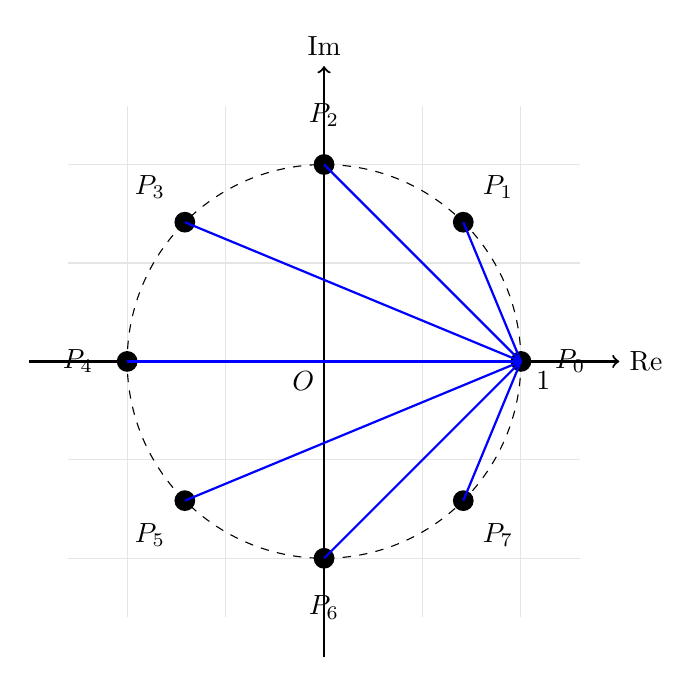
\begin{tikzpicture}[scale=2.5]
    % Grid and Axes
    \draw[gray!20, thin, step=0.5] (-1.3,-1.3) grid (1.3,1.3);
    \draw[->, thick] (-1.5,0) -- (1.5,0) node[right] {Re};
    \draw[->, thick] (0,-1.5) -- (0,1.5) node[above] {Im};
    \draw[dashed] (0,0) circle (1);
    
    % Vertices for 2n = 8 (n=4)
    \foreach \k in {0,1,...,7} {
        \coordinate (P\k) at ({\k*360/8}:1);
        \fill (P\k) circle (1.5pt);
        \node at ({\k*360/8}:1.25) {$P_{\k}$};
    }
    
    % Chords from P0 to all other vertices
    \foreach \k in {1,2,...,7} {
        \draw[blue, thick] (P0) -- (P\k);
    }
    
    % Label Origin and P0
    \node[anchor=north east] at (0,0) {$O$};
    \node[anchor=north west, xshift=2pt] at (P0) {$1$};
\end{tikzpicture}
\end{center}
\end{solution}

\begin{takeaways}
\begin{enumerate}
    \item Geometrically, $|1 - e^{i\frac{k\pi}{n}}|$ represents the distance between the vertex $P_0$ (at $1+0i$) and every other vertex $P_k$ of a regular $2n$-gon inscribed in the unit circle.
    \item \textbf{Geometric Product:} The product of all chord lengths from one vertex in a regular $m$-gon is exactly $m$.
    \item \textbf{Trigonometric Identity:} This problem proves $\prod_{k=1}^{2n-1} \sin\left(\frac{k\pi}{2n}\right) = \frac{2n}{2^{2n-1}}$.
    \item \textbf{Complex-Geometric Connection:} Polynomial factorization over roots of unity directly yields geometric properties of regular polygons.
    \item \textbf{Modulus of Products:} The identity $|z_1 z_2| = |z_1||z_2|$ is essential for connecting algebraic and geometric interpretations.
    \item Try proving (iv) using induction as an alternative method (?) or without using complex numbers (?)
\end{enumerate}
\end{takeaways}
